%!TEX root = /Users/stevenmartell/Documents/iSCAM-project/fba/Halibut/WRITEUP/Halibut.tex
\section{Methods} % (fold)
\label{sec:methods}

Details of the simulation model are documented in Appendix \ref{sec:model_description}.  In short, the simulation model is a sex- and age-structured population dynamics model were the initial 1996 age-structure and age-1 recruits from 1996-2006 is based on the IPHC assessment conducted by \cite{Hare2012Rara}.  Total mortality rates for the 1996-2011 period were based on the same values estimated in the IPHC assessment and historical and simulated weight-at-age data is based on the mean length-at-age data  for males and females  in the setline survey.  

Future projections were based on poor, average, and good recruitment (defined as $\pm$60\% in average recruitment).  Growth was modelled either as density-independent, or density-dependent where the asymptotic length of halibut would decrease with increasing cohort density, and vice versa.  It was assumed that selectivity in the directed commercial fishery remained unchanged in all future simulations.  Selectivity is a function of length, and therefore, with decreasing mean size-at-age the fishery would target older fish.  The length-based selectivity function was based on the same piece-wise linear function where fish less than 60 cm have a selectivity of 0 and fish greater than 120 cm were fully vulnerable.  

Additional model assumptions include a fixed natural mortality rate for each sex, the coefficient of variation in length-at-age is 0.1, the discard mortality rate in the directed fishery is 0.17 per year, and all future catches are based on the constand harvest rate policy (0.215, or 0.16 depending on area).  Area specific biomass apportionment is based on the 2011 apportionment values, and discard rates for O32 and U32 fish are carried forward from the 2011 realized values. The price per pound is based on prices in Homer Alaska, 10-20lbs at \$6.75, 20-40lbs at \$7.35 and 40+lbs at \$7.50.  An assumed price of \$5.00 per for fish in the length interval of 66cm to 81cm was adopted to calculate the value of the wastage or value of fish less than 81 cm.  The definition of wastage for this simulation is the amount of fish (in lbs) that is caught but is less than the minimum size limit and is assumed to die.

\subsection{Joint probability model for retention} % (fold)
\label{sub:joint_probability_model_for_retention}
The probability of capturing a fish in a given size interval $x$ is a property of the selectivity of the fishing gear and the number of available fish in the size interval ($x$).  This simulation model, and the IPHC assessment model, does not model the number of fish at length explicitly; rather, the accounting system is based on the numbers-at-age.  The estimated selectivity function is based on length, and the probability of capturing a fish of a given age is approximated by the mean length-at-age in a given year. In the IPHC assessment model, a series of selectivity coefficients are estimated for the length intervals 60,70, $\ldots$, 120 and the probability of capturing a fish of a given age is a function of the mean length-at-age. With variable growth rates the probability of capturing a fish of a given age can change from year to year with changes in fish size.  As fish grow slower, the age at recruitment to the fishery shift to an older age.

The probability of retaining a fish of a given age $j$ is also a function of the mean length-at-age and the minimum size limit.   Therefore the probability of capturing  a fish of a given age and keeping it ($p(c_j)$) is a joint probability model that can be defined as follows:
\[p(c_j) = p(j) \cdot p(r_j),\]
where $p(j)$ is the probability of capturing a fish of age $j$, and $p(r_j)$ is the probability of retaining a fish of age $j$.  The probability of capture $p(j)$ is the piece-wise linear interpolation of the mean length-at-age (length-based selectivity), and the probability that an individual age-$j$ fish is greater than the minimum size limit is:
\[p(r_j) = \int_{l_j=\mathrm{MSL}}^{l_j=\infty}
\frac{1}{\sqrt{2\pi}\sigma_j} \exp\left[-\frac{(l_j-\mathrm{MSL})^2}{2\sigma_j^2}  \right] dl_j
\]
where MSL is the minimum size limit, $l_j$ is the mean length-at-age $j$, and $\sigma_j$ is the standard deviation in the mean length-at-age.  To approximate the above integral, a logistic function was used with a mean (50\% probability of capture) corresponding to the MSL, and the standard deviation based on a CV of 0.1 for the mean length-at-age.

The probability of a fishing dying at a given age is then the probability of capturing a fish of a given age $j$ times the probability of retention times the probability of discarding ($1-p(r_j)$) the fish times the discard mortality rate:
\[
p(h_j) = p(j) [p(r_j) (1-p(r_j))d],
\]
where $d$ is the discard mortality rate.

% subsection joint_probability_model_for_retention (end)

\subsection{Simulation scenarios} % (fold)
\label{sub:simulation_scenarios}
Three alternative size-limit policy options were explored, the status quo policy of 32 inch size limit, and a 29 and 26 inch size limit (Figure \ref{fig:FIGURES_SIZELIMIT_SelRetA}).  For each of the policy options, a total of 6 simulation runs were performed with poor, average, and good recruitment under two alternative hypotheses about future growth of halibut.  These scenarios are summarized in the form of a graphical decision table where the rows of the table correspond to alternative growth models, and the columns correspond to alternative size limit policies.
\begin{figure}[htbp]
	\centering
		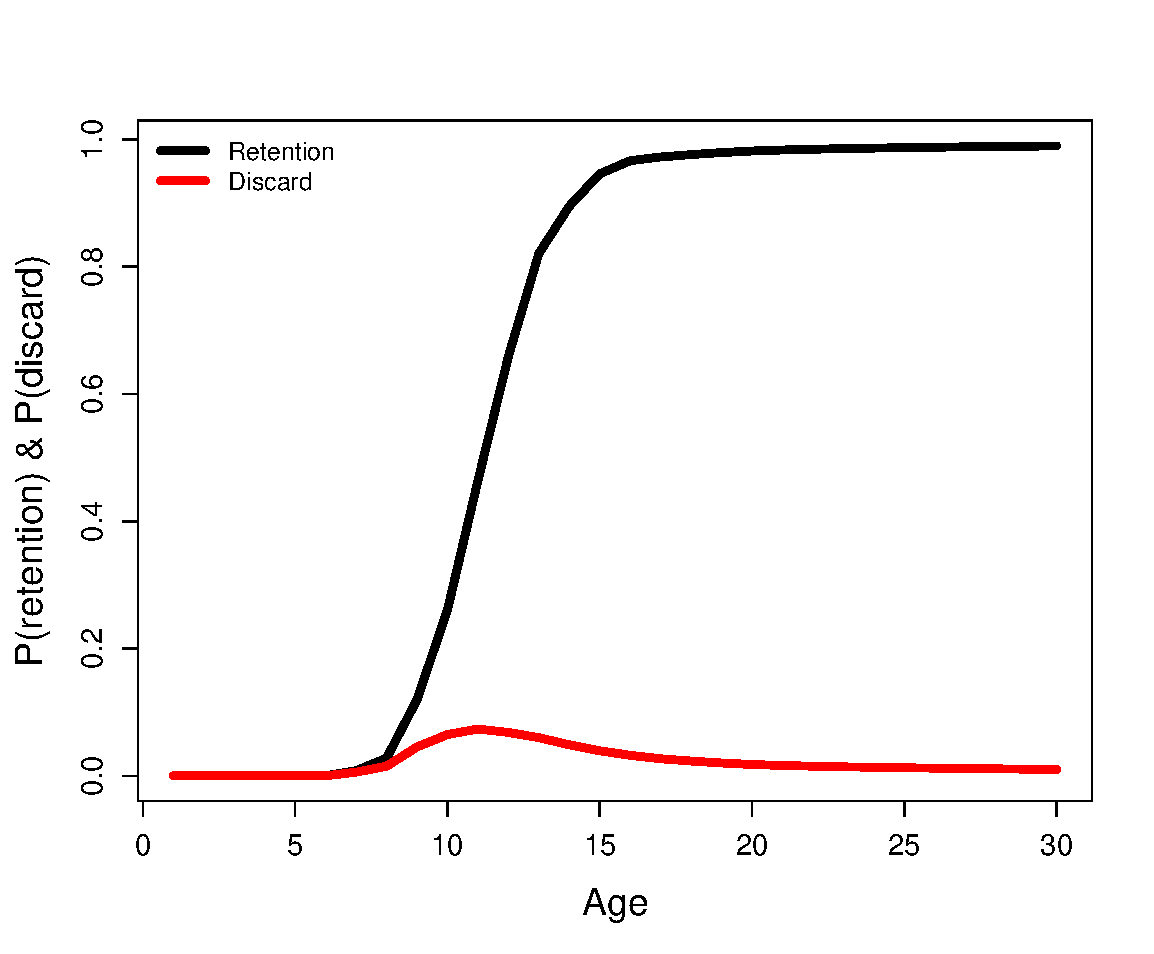
\includegraphics[height=1.5in]{../FIGURES/SIZELIMIT/SelRetA.pdf}
		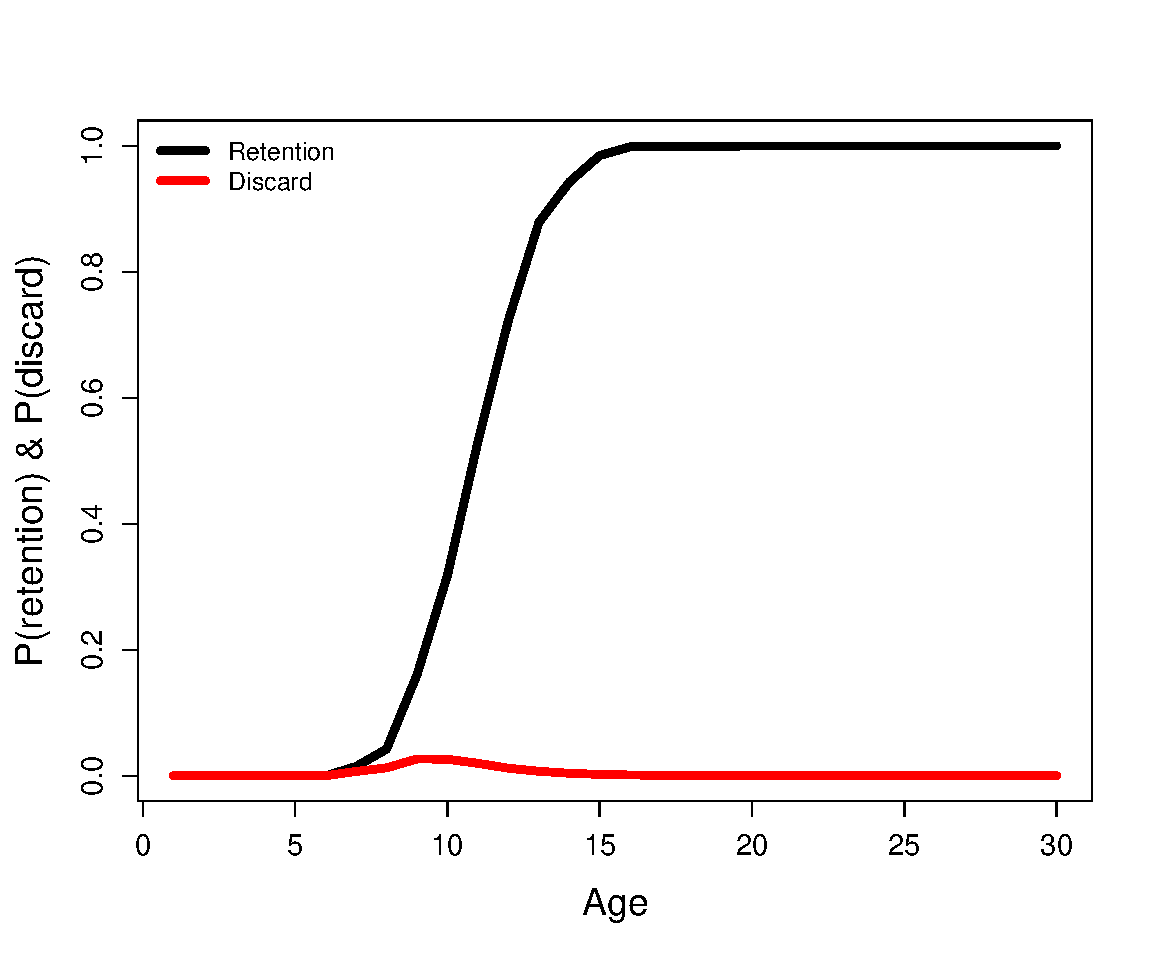
\includegraphics[height=1.5in]{../FIGURES/SIZELIMIT/SelRetC.pdf}
		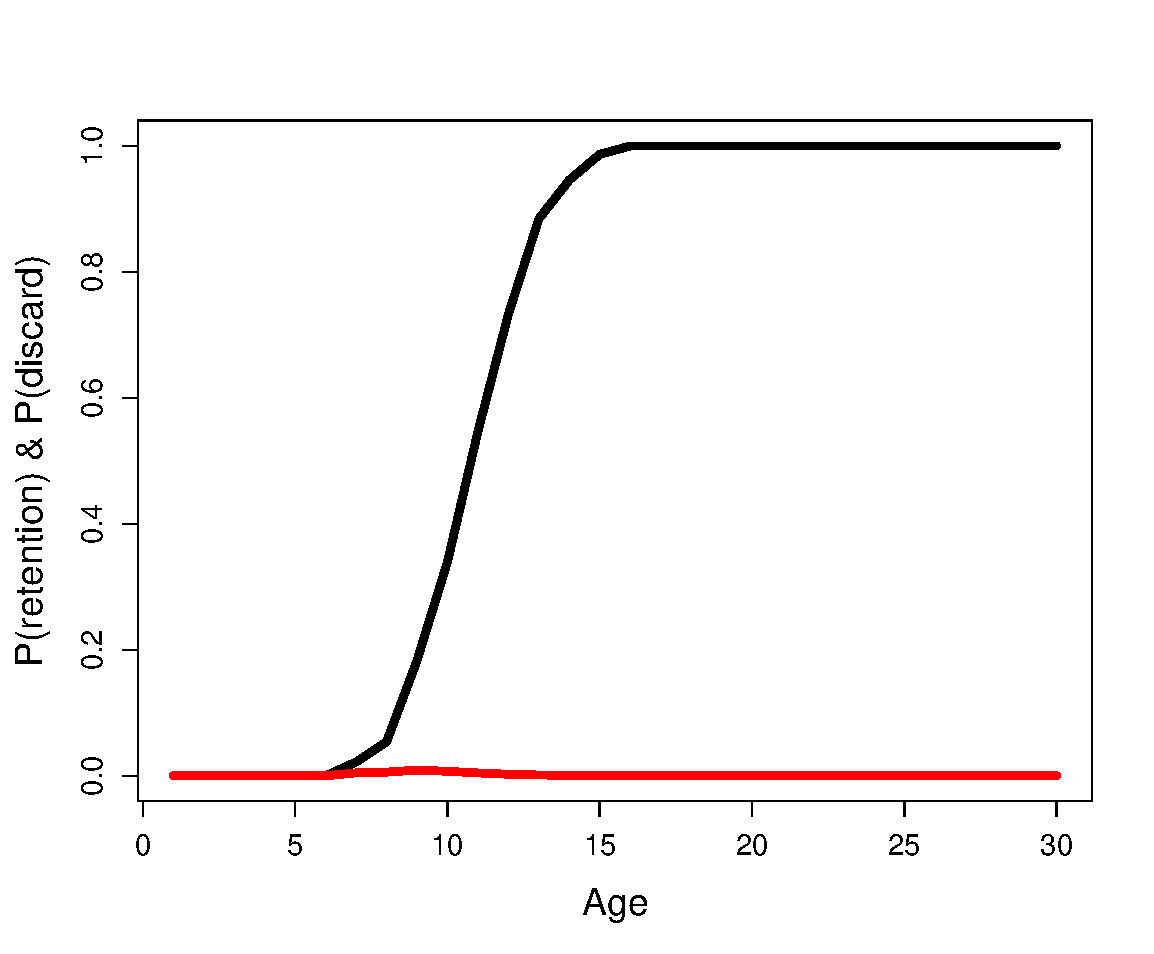
\includegraphics[height=1.5in]{../FIGURES/SIZELIMIT/SelRetB.pdf}
	\caption{Example of retention- and discard-at-age probabilities for a given growth curve over 32 inch (left) 29 inch (middle) and 26 inch (right) minimum size limit.}
	\label{fig:FIGURES_SIZELIMIT_SelRetA}
\end{figure}



% subsection simulation_scenarios (end)

% section methods (end)















